%%%%%%%%%%%%%%%%%%%%%%%%%%%%% Define Article %%%%%%%%%%%%%%%%%%%%%%%%%%%%%%%%%%
\documentclass{article}
%%%%%%%%%%%%%%%%%%%%%%%%%%%%%%%%%%%%%%%%%%%%%%%%%%%%%%%%%%%%%%%%%%%%%%%%%%%%%%%

%%%%%%%%%%%%%%%%%%%%%%%%%%%%% Using Packages %%%%%%%%%%%%%%%%%%%%%%%%%%%%%%%%%%
\usepackage{geometry}
\usepackage{graphicx}
\usepackage{amssymb}
\usepackage{amsmath}
\usepackage{amsthm}
\usepackage{empheq}
\usepackage{mdframed}
\usepackage{booktabs}
\usepackage{lipsum}
\usepackage{enumitem}
\usepackage{graphicx}
\usepackage{color}
\usepackage{psfrag}
\usepackage{pgfplots}
\usepackage{bm}
\usepackage[spanish]{babel}
%%%%%%%%%%%%%%%%%%%%%%%%%%%%%%%%%%%%%%%%%%%%%%%%%%%%%%%%%%%%%%%%%%%%%%%%%%%%%%%

% Other Settings

%%%%%%%%%%%%%%%%%%%%%%%%%% Page Setting %%%%%%%%%%%%%%%%%%%%%%%%%%%%%%%%%%%%%%%
\geometry{a4paper,margin=1.2in}

%%%%%%%%%%%%%%%%%%%%%%%%%% Define some useful colors %%%%%%%%%%%%%%%%%%%%%%%%%%
\definecolor{ocre}{RGB}{243,102,25}
\definecolor{mygray}{RGB}{243,243,244}
\definecolor{deepGreen}{RGB}{26,111,0}
\definecolor{shallowGreen}{RGB}{235,255,255}
\definecolor{deepBlue}{RGB}{61,124,222}
\definecolor{shallowBlue}{RGB}{235,249,255}
%%%%%%%%%%%%%%%%%%%%%%%%%%%%%%%%%%%%%%%%%%%%%%%%%%%%%%%%%%%%%%%%%%%%%%%%%%%%%%%

%%%%%%%%%%%%%%%%%%%%%%%%%% Define an orangebox command %%%%%%%%%%%%%%%%%%%%%%%%
\newcommand\orangebox[1]{\fcolorbox{ocre}{mygray}{\hspace{1em}#1\hspace{1em}}}
%%%%%%%%%%%%%%%%%%%%%%%%%%%%%%%%%%%%%%%%%%%%%%%%%%%%%%%%%%%%%%%%%%%%%%%%%%%%%%%

%%%%%%%%%%%%%%%%%%%%%%%%%%%% English Environments %%%%%%%%%%%%%%%%%%%%%%%%%%%%%
\newtheoremstyle{mytheoremstyle}{3pt}{3pt}{\normalfont}{0cm}{\rmfamily\bfseries}{}{1em}{{\color{black}\thmname{#1}~\thmnumber{#2}}\thmnote{\,--\,#3}}
\newtheoremstyle{myproblemstyle}{3pt}{3pt}{\normalfont}{0cm}{\rmfamily\bfseries}{}{1em}{{\color{black}\thmname{#1}~\thmnumber{#2}}\thmnote{\,--\,#3}}
\theoremstyle{mytheoremstyle}
\newmdtheoremenv[linewidth=1pt,backgroundcolor=shallowGreen,linecolor=deepGreen,leftmargin=0pt,innerleftmargin=20pt,innerrightmargin=20pt,]{theorem}{Theorem}[section]
\theoremstyle{mytheoremstyle}
\newmdtheoremenv[linewidth=1pt,backgroundcolor=shallowBlue,linecolor=deepBlue,leftmargin=0pt,innerleftmargin=20pt,innerrightmargin=20pt,]{definition}{Definition}[section]
\theoremstyle{myproblemstyle}
\newmdtheoremenv[linecolor=black,leftmargin=0pt,innerleftmargin=10pt,innerrightmargin=10pt,]{problem}{Problem}[section]
%%%%%%%%%%%%%%%%%%%%%%%%%%%%%%%%%%%%%%%%%%%%%%%%%%%%%%%%%%%%%%%%%%%%%%%%%%%%%%%

%%%%%%%%%%%%%%%%%%%%%%%%%%%%%%% Plotting Settings %%%%%%%%%%%%%%%%%%%%%%%%%%%%%
\usepgfplotslibrary{colorbrewer}
\pgfplotsset{width=8cm,compat=1.9}
%%%%%%%%%%%%%%%%%%%%%%%%%%%%%%%%%%%%%%%%%%%%%%%%%%%%%%%%%%%%%%%%%%%%%%%%%%%%%%%

%%%%%%%%%%%%%%%%%%%%%%%%%%%%%%% Title & Author %%%%%%%%%%%%%%%%%%%%%%%%%%%%%%%%
\title{Certamen 1 Introducción a la prospección remota}
\author{Alex Villarroel Carrasco}
%%%%%%%%%%%%%%%%%%%%%%%%%%%%%%%%%%%%%%%%%%%%%%%%%%%%%%%%%%%%%%%%%%%%%%%%%%%%%%%

\begin{document}
\usetikzlibrary{positioning}
	\tikzset{every picture/.style={line width=0.75pt}}    
	\pagestyle{plain}
	\begin{flushleft}
		Departamento de Geofísica \hfill Introducción a prospección geofísica\\
		Facultad de Cs. Físicas y Matemáticas\\
		\underline{Universidad de Concepción}
	\end{flushleft}
	
	\begin{flushright}\vspace{-5mm}
		
\includegraphics[height=1.5cm]{escudo.png}
	\end{flushright}
	
	\begin{center}\vspace{-1cm}
		\textbf{\large Certamen 01 de introducción a prospección geofísica}\\
		{\textcolor{blue}{Alex Villarroel Carrasco}}\\
	\end{center}
	\rule{\linewidth}{0.1mm}
	\\
    \section*{Pregunta 1}
	 1. De las imágenes respectivas para cada caso (2 casos: 1\_PELEHUE y 10\_PELEHUE)
		“picar” una primera llegada para cada geófono, siempre que resulte adecuado
		hacerlo. Construir una tabla con tiempo vs d istancia. Recordar considerar la
		distancia igual a cero (0) el punto del “shot point” respectivo.
	\section*{Respuesta}
	A partir de los archivos entregados por el profesor, se realizó el manejo de datos mediante Obspy, para rehacer un plot de distancia vs tiempo.
	\begin{figure*}[h]
		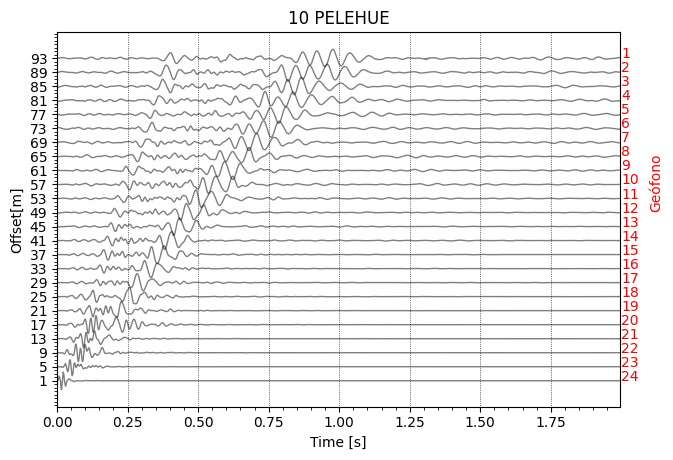
\includegraphics[width=\textwidth]{/home/alex/Desktop/Prospeccion-geofisica/Cert1/1PELEHUE.png}
		\caption{Section plot de 1 PELEHUE, shot point a un metro del geófono 1}
	\end{figure*}
	\begin{figure*}[h]
		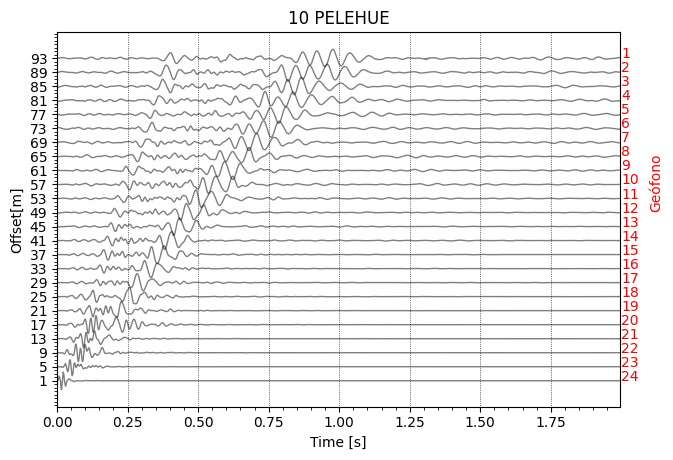
\includegraphics[width=\textwidth]{/home/alex/Desktop/Prospeccion-geofisica/Cert1/10Pelehue.png}
		\caption{Section plot de 10 PELEHUE, shot point a un metro del geófono 24}
	\end{figure*}
	\begin{figure*}[h]
		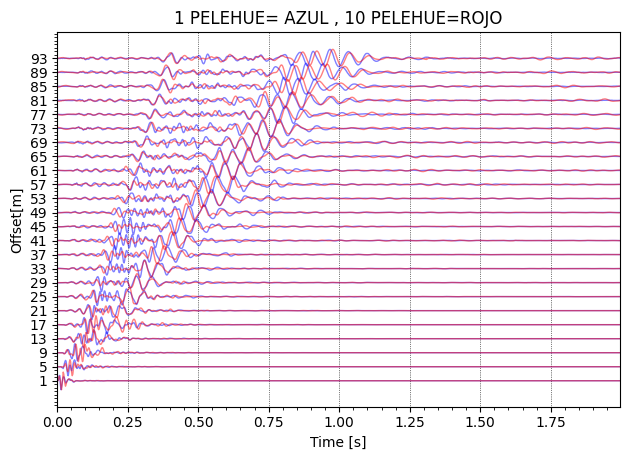
\includegraphics[width=\textwidth]{/home/alex/Desktop/Prospeccion-geofisica/Cert1/ambos.png}
		\caption{Section plot de 10 PELEHUE, shot point a un metro del geófono 24}
	\end{figure*}
	\newpage
	A partir los gráficos, y con la ayuda de la herramienta \textbf{SeisGram2K}, se realizó el picado correspondiente a cada shot point
	\\% Please add the following required packages to your document preamble:
	
% \usepackage[table,xcdraw]{xcolor}
% If you use beamer only pass "xcolor=table" option, i.e. \documentclass[xcolor=table]{beamer}
	\begin{tabular}{|c|c|c|}
	\hline
	\textbf{Geófono} & \textbf{\begin{tabular}[c]{@{}c@{}}Tiempo de \\ llegada {[}min.s{]}\end{tabular}} & \textbf{\begin{tabular}[c]{@{}c@{}}Distancia \\ del shotpoint\\ {[}m{]}\end{tabular}} \\ \hline
	1                & 35.350                                                                            & 93                                                                                    \\ \hline
	2                & 35.329                                                                            & 89                                                                                    \\ \hline
	3                & 35.322                                                                            & 85                                                                                    \\ \hline
	4                & 35.320                                                                            & 81                                                                                    \\ \hline
	6                & 35.286                                                                            & 77                                                                                    \\ \hline
	5                & 35.281                                                                            & 73                                                                                    \\ \hline
	7                & 35.275                                                                            & 69                                                                                    \\ \hline
	8                & 35.260                                                                            & 65                                                                                    \\ \hline
	9                & 35.232                                                                            & 61                                                                                    \\ \hline
	10               & 35.219                                                                            & 57                                                                                    \\ \hline
	11               & 35.196                                                                            & 53                                                                                    \\ \hline
	12               & 35.188                                                                            & 49                                                                                    \\ \hline
	13               & 35.179                                                                            & 45                                                                                    \\ \hline
	14               & 35.169                                                                            & 41                                                                                    \\ \hline
	15               & 35.148                                                                            & 37                                                                                    \\ \hline
	16               & 35.142                                                                            & 33                                                                                    \\ \hline
	17               & 35.122                                                                            & 29                                                                                    \\ \hline
	18               & 35.084                                                                            & 25                                                                                    \\ \hline
	19               & 35.084                                                                            & 21                                                                                    \\ \hline
	21               & 35.033                                                                            & 17                                                                                    \\ \hline
	20               & 35.030                                                                            & 13                                                                                    \\ \hline
	22               & 35.026                                                                            & 9                                                                                     \\ \hline
	23               & 35.024                                                                            & 5                                                                                     \\ \hline
	24               & 35.003                                                                            & 1                                                                                     \\ \hline
	\end{tabular}


		\begin{tabular}{|c|c|c|}
		\hline
		\textbf{Geófono} &
		  \textbf{\begin{tabular}[c]{@{}c@{}}Tiempo de \\ llegada {[}min.s{]}\end{tabular}} &
		  \textbf{\begin{tabular}[c]{@{}c@{}}Distancia \\ del shotpoint\\ {[}m{]}\end{tabular}} \\ \hline
		1  & 12.003 & 1  \\ \hline
		2  & 12.015 & 5  \\ \hline
		3  & 12.022 & 9  \\ \hline
		4  & 12.026 & 13 \\ \hline
		5  & 12.033 & 17 \\ \hline
		6  & 12.060 & 21 \\ \hline
		7  & 12.117 & 25 \\ \hline
		8  & 12.127 & 29 \\ \hline
		9  & 12.149 & 33 \\ \hline
		10 & 12.160 & 37 \\ \hline
		11 & 12.169 & 41 \\ \hline
		13 & 12.181 & 45 \\ \hline
		12 & 12.194 & 49 \\ \hline
		14 & 12.227 & 53 \\ \hline
		15 & 12.235 & 57 \\ \hline
		16 & 12.256 & 61 \\ \hline
		17 & 12.266 & 65 \\ \hline
		18 & 12.269 & 69 \\ \hline
		19 & 12.294 & 73 \\ \hline
		20 & 12.312 & 77 \\ \hline
		21 & 12.319 & 81 \\ \hline
		22 & 12.325 & 85 \\ \hline
		23 & 12.347 & 89 \\ \hline
		24 & 12.357 & 93 \\ \hline
		\end{tabular}
	\end{document}